\section{Com funcionen els dispositius electrònics}
Els dispositius electrònics com els telèfons mòbils, tauletes, ordinadors, caixers automàtics, consoles, impressores, rentaplats, televisors, rentadores... tots resolen tasques diferents i tenen utilitats diferents, però, tots tenen els components necessaris per executar un programa.

\subsection{Com interactuem amb els dispositius electrònics}
Els dispositius són màquines que responen a accions com ara tocar la pantalla tàctil, clicar amb el ratolí, escriure amb el teclat, parlar pel micròfon, prémer algun botó del comandament a distància... i, el dispositiu genera una resposta en funció de l'acció de l'usuari: pot canviar el contingut de la pantalla, reproduir un so a través dels altaveus, enviar un senyal a un altre dispositiu, canviar el canal del televisor, retirar una quantitat de diners...

La informació que l'usuari dona al dispositiu l'anomenarem \textbf{entrada}. I al resultat o resposta que genera l'anomenarem \textbf{sortida}. 

Per exemple, quan premem el botó d'incrementar el volum del comandament del televisor, generem una entrada. El televisor la processa i genera una sortida: incrementa el volum. Si l'entrada fos diferent i premem el botó de canviar de canal, la sortida també seria diferent, i s'hauria canviat el canal en lloc d'incrementar el volum. Per tant, podem deduir que la sortida depèn completament de l'entrada. Si canviem l'entrada, la sortida també serà diferent.

El maquinari dels dispositius per si mateixos no poden processar les entrades i generar sortides, necessiten que algun element rebi la informació (entrada), la processi i generi el resultat (sortida). Aquí és on entra la programació. Els programes reben, llegeixen i processen la informació de l'entrada i generen la sortida.

Per exemple, premem el botó d'engegar del mòbil (\textbf{entrada}), l'entrada arriba al \textbf{programa}, aquest processa la informació i genera una \textbf{sortida}, la qual consisteix a encendre la pantalla.

\begin{figure}[h]
    \centering
    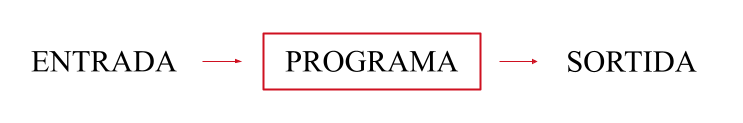
\includegraphics[width=.7\textwidth]{capitols/figures/i_o prog.png}
    \caption[Diagrama d'entrada, programa i sortida.]{Diagrama d'entrada, programa i sortida. Font: elaboració pròpia.}
    \label{Figura}
\end{figure}

Totes les tasques que podem resoldre utilitzant un programa les anomenarem problema. Ens referim a tots els exemples d'aquest punt com a un problema que hem resolt amb un programa. 

Quan parlem d'un problema matemàtic com ara sumar dos nombres, la solució és el resultat de la suma, l'equivalent a la sortida. Però quan parlem de problemes de programació, com els d'aquest treball, la solució és el procediment, el qual és diferent de la sortida, ja que la sortida és el resultat de finalitzar el procediment.

\subsection{Què són els algoritmes i en què es diferencien dels programes}
Un algoritme és un procediment, un seguit de passos finits i ordenats que resolen un problema concret. Els algoritmes ofereixen formes teòriques de resoldre un problema.

En canvi, un programa és tot allò que un ordinador pot entendre i executar. Un programa pot implementar\footnote{La paraula 'implementar' s'utilitza en aquest context per expressar l'acció de passar alguna solució/procediment/algoritme a un programa. La implementació d'un algoritme és un programa que resolgui la mateixa tasca que l'algoritme implementat.} o \quotes{traduir} un algoritme. Els programes ofereixen formes pràctiques de resoldre un problema.

És a dir, els algoritmes són els procediments o els passos a seguir. I els programes són la traducció dels algoritmes de manera que els dispositius els puguin executar.

Posem com a exemple el següent problema que volem resoldre amb un programa: definim tres nombres com a $x, y, z$ i volem trobar $(x+y)\cdot z$. Aquest problema està generalitzat perquè no tenim valors fixos per l'entrada i, per tant, no podem saber quina és la sortida. És a dir, farem un algoritme i programa que funcionin per a qualsevol nombre, no només per a un.

Per solucionar matemàticament aquest problema, primer cal resoldre la suma, i després la multiplicació. I per fer un programa que el resolgui, podríem fer el següent:

ALGORITME:
\begin{enumerate}
    \item Llegir els nombres amb l'ordre adequat.
    \item Sumar els dos primers nombres.
    \item Multiplicar el resultat del pas 2 pel tercer nombre.
    \item La solució és el resultat del pas 3.
\end{enumerate}

PROGRAMA:
\begin{figure}[h]
    \begin{minted}[
    frame=lines,
    framesep=2mm,
    baselinestretch=1.2,
    bgcolor=LightGray,
    fontsize=\footnotesize,
    linenos
    ]{python}
    x = int(input())    # agafar l'entrada i assignar-li el valor x
    y = int(input())    # agafar l'entrada i assignar-li el valor y
    z = int(input())    # agafar l'entrada i assignar-li el valor z
    
    a  = x + y          # pas 2 de l'algoritme
    b = a * z           # pas 3 de l'algoritme
    print(b)            # escriure la solució
    \end{minted}
    \caption[Programa que resol l'operació.]{Programa que resol l'operació\footnotemark. Font: elaboració pròpia.}
    \label{Figura}
\end{figure}
\footnotetext{El programa està escrit en Python. El propòsit és fer-se una idea de com és un programa, ja que en parlarem durant tot el treball. No cal entendre la sintaxi del llenguatge de programació. Després dels coixinets hi ha un comentari explicatiu que no afecta el funcionament.}

Com podem veure, l'algoritme és un seguit de passos i el programa permet executar-lo en un dispositiu, ja que l'escriu de forma que aquests el poden executar.

\newpage Veiem com independentment de les entrades que tinguem, el procediment sempre serà el mateix. En un cas generalitzat com aquest, no tenim entrades i sortides concretes, però podem especificar un cas i d'aquesta manera podem comprovar el correcte funcionament del programa. Posaré un cas concret en què $x = 2, y = 3, z = 4$. En aquest cas, les entrades són 2, 3 i 4 i la sortida seria $(2+3)\cdot4 = 20$.

\subsection{Com se solucionen els problemes més complexos}
En els exemples anteriors hem resolt problemes molt senzills, però quan hem d'abordar problemes més complexos, ens trobem amb altres dificultats. Pot passar que hi hagi moltes solucions diferents que resolen el problema, i hi haurà solucions poc eficients que haurem d'identificar i descartar. És molt important analitzar l'eficiència de les solucions per saber si és profitós implementar-les i executar-les.

Precisament en aquest treball ens centrarem a trobar diverses solucions per a un problema i analitzar-les per saber la seva complexitat en funció de la quantitat de dades de l'entrada. Ho explicaré més detalladament en el següent apartat. Ara per fer-nos una idea que un problema té diverses solucions unes més eficients que les altres, posaré un exemple:

El problema consisteix a fer un programa que trobi la solució a qualsevol sudoku\footnote{Aquest és un trencaclosques en què l'objectiu és omplir amb nombres de l'1 al 9 una quadrícula de 9x9 caselles dividida en quadres de 3x3. Les úniques restriccions són que no es poden repetir nombres en cap filera, columna o quadre 3x3. Inicialment, el trencaclosques et proporciona alguns nombres col·locats a la seva casella corresponent i l'objectiu és trobar-ne la resta.}. Hi ha moltes estratègies que es poden seguir per resoldre'n un, seguidament en proposo dues. 

La primera estratègia és posar tots els nombres a l'atzar i comprovar cada vegada si la solució és vàlida, i repetir el procés fins a trobar la combinació correcta. Quan apliquem aquest algoritme en un programa, aquest serà poc eficient, perquè hi ha moltes combinacions possibles, i inclús podríem repetir combinacions que ja hem provat.

La segona estratègia és la següent: Posem un nombre escollit de forma ordenada en una casella buida. Seguidament, comprovem que la fila, columna, i el quadre ens ho permet, en el cas que sigui vàlid, repetim el procés amb la següent casella buida, i, si no és vàlid, provem amb un nombre diferent. Amb aquesta solució estem provant nombres de forma ordenada i sense repetir-los. Aquesta solució la podem generalitzar de la següent manera: si funciona avancem un pas i repetim el procés, si no funciona retrocedim i repetim el procés provant el següent nombre. Aquest tipus de solució és un algoritme de \textit{backtracking}. La implementació d'aquesta solució es pot veure a l'annex 6.1.

\section{Quina és la millor solució?}
Quan podem solucionar un mateix problema de diverses maneres, el més lògic és resoldre'l de la manera més eficient possible. Si no, totes les tasques tardarien molt més en acabar i el resultat seria un dispositiu poc eficient. Per evitar això hem d'analitzar l'eficiència dels algoritmes.

\subsection{Introducció a l'anàlisi de l'eficiència dels algoritmes}%----------------------------------------
L'eficiència dels algoritmes o complexitat algorítmica és una mesura per determinar el cost d'un algoritme o programa. Amb aquesta mesura podem comparar els algoritmes o programes entre ells i determinar quin és més convenient d'utilitzar. La complexitat algorítmica depèn únicament de dos paràmetres que s'estudien per separat:
\begin{enumerate}
    \item L'\textbf{eficiència espacial} (la quantitat de memòria que ocupa).
    \item L'\textbf{eficiència temporal} (la velocitat de l'algoritme).
\end{enumerate}

L'eficiència espacial fa referència a l'espai que ocupen les dades, les dades d'entrada s'han d'emmagatzemar perquè el programa les pugui utilitzar (bases de dades), i l'algoritme pot requerir emmagatzemar-ne més. Com més dades s'hagin d'emmagatzemar diem que l'algoritme té una pitjor eficiència espacial o major complexitat. Però en aquest treball no ens centrarem en aquesta part de l'estudi de l'eficiència.

Ens centrarem en l'eficiència temporal, la qual mesura el cost que té un algoritme o programa en funció de la mida de l'entrada. 

Per exemple: un dentista tarda 30 minuts per visitar cada pacient. Per tant, per saber quan acabarà la jornada només hem de multiplicar el nombre de pacients per 30 minuts. Si anomenem $n$ el nombre de pacients, podem saber que el dentista treballarà $30 \cdot n$ minuts. D'aquesta manera estem expressant en funció del nombre de pacients ($n$) el temps que treballarà el dentista en una jornada.

L'eficiència temporal mesura el mateix. En funció de la quantitat de dades de l'entrada ($n$), expressa quant tardarà l'algoritme o programa en acabar.

L'eficiència temporal es pot analitzar de dues formes:
\begin{enumerate}
    \item De forma \textbf{matemàtica}. Consisteix a analitzar la quantitat d'operacions que fa l'algoritme.
    \item De forma \textbf{empírica}. Consisteix a implementar l'algoritme i mesurar el temps que tarda el programa. A partir d'aquestes mesures s'intenta predir el comportament del programa, i, per tant, de l'algoritme, per les mesures no realitzades.
\end{enumerate}

Ha de quedar clar que l'eficiència temporal d'un algoritme no depèn en absolut de l'ordinador que utilitzem, sinó de l'algoritme en si mateix, és a dir, en la quantitat d'operacions o comparacions que faci. Un ordinador més potent podrà fer les operacions més ràpidament que un de més lent, però els dos faran la mateixa quantitat d'operacions, és a dir, serà més ràpid, però no més eficient.

Tornant a l'exemple del dentista, si un dentista B tarda 5 minuts per pacient en lloc del dentista A que en tarda 30. El dentista B tardarà $5 \cdot n$ minuts a atendre $n$ pacients. El dentista B atén més ràpidament els pacients, però els dos realitzen el mateix procediment. Per tant, el dentista B és més ràpid, però, en termes d'anàlisi d'eficiència tots dos són igual d'eficients. 

L'anàlisi empírica és poc fiable, ja que depèn de les dades d'entrada i de l'entorn de programació utilitzat. En canvi, en l'anàlisi matemàtica podem extreure conclusions basant-nos únicament en l'algoritme i no en les implementacions d'aquest. A més, un dels objectius principals d'analitzar l'eficiència dels algoritmes és determinar si és profitós implementar-lo, i això únicament es pot fer de forma teòrica analitzant l'algoritme.

\begin{figure}[H]
    \centering
    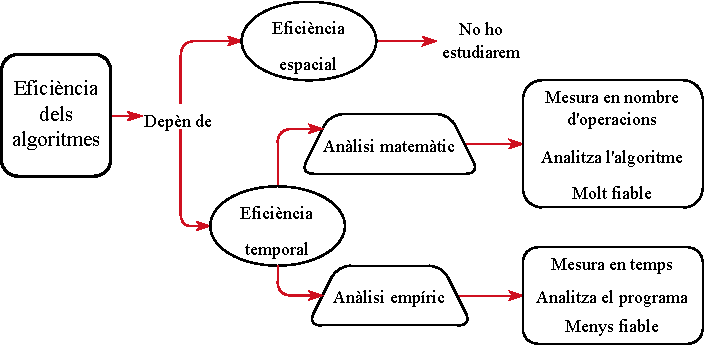
\includegraphics[width=.8\textwidth]{capitols/figures/diagram.drawio (1).pdf}
    \caption[Diagrama de l'eficiència dels algoritmes.]{Diagrama de l'eficiència dels algoritmes. Font: elaboració pròpia.}
    \label{Figura}
\end{figure}

\subsection{Notació de Landau}
Hi ha diverses maneres de mesurar la complexitat algorítmica respecte de l'entrada. La notació de Landau engloba tres notacions, $O()$, $\theta()$ i $o()$. En aquest treball només definirem i estudiarem $O()$.

La notació de Landau és una notació asimptòtica que proporciona una forma matemàtica d'expressar la complexitat d'un algoritme en funció d'$n$ quan $n$ pren valors molt grans. Aquest anàlisis és totalment independent de la implementació de l'algoritme.

Definim $O(g)$ com el conjunt de funcions que per a valors molt grans d'$n$ (asimptòticament) creixen de manera proporcional o inferior a la funció $g$. Per tant, $f \in O(g) \iff f = O(g)$.

Per exemple, $f(n) = 5n^2 - 2n$ com que $f(n) \in O(n^2)$ podem afirmar que $5n^2 - 2n = O(n^2)$. 

Si ens hi fixem, estem perdent informació de la funció $g(n)$, ja que $O(n^2)$ engloba totes les funcions de creixement inferior i proporcional a $n^2$. Això ens permet ignorar detalls com les constants o les funcions de menor ordre que no són rellevants en l'anàlisi de l'eficiència dels algoritmes.

Propietats d'$O()$ (només les necessàries per aquest treball):
\begin{enumerate}
    \item $O(f) \cdot O(g) = O(f \cdot g)$
    \item $O(f) + O(g) = O(f + g) = O(Max\{f,g\})$
\end{enumerate}

A l'hora d'analitzar l'eficiència dels algoritmes, ens interessa saber de quina manera creix l'algoritme en funció a la mida de l'entrada. També ens interessa analitzar el pitjor cas possible, d'aquesta manera podem saber que en qualsevol altre cas, l'algoritme tindrà un cost menor o igual que en el cas analitzat.

El pitjor cas possible fa referència a l'entrada que perjudica més el funcionament d'aquell algoritme concret. El pitjor cas possible és diferent per a cada algoritme i n'hi ha que no en tenen.

Cal remarcar que $O(g)$ no és el nombre d'operacions que realitza un algoritme en el pitjor cas possible. Si no que a partir d'analitzar el nombre d'operacions $f$, $f = O(g) \iff f \in O(g)$. 

Seguidament, explicaré les quatre complexitats més comunes que són les que tenen afectació en l'elaboració d'aquest treball.

\subsubsection*{Constant $O(1)$}
En aquest cas a l'interior dels parèntesis no hi ha cap $n$, això vol dir que les operacions no depenen de la mida de l'entrada i sempre, independentment de la seva mida l'algoritme farà la mateixa quantitat d'operacions.

Per exemple, si agafem un llibre d'un prestatge d'$n$ llibres i saps que vols el primer. No caldrà que el busquis, podràs agafar el primer fent una única operació. No importa quants llibres hi hagi, sempre faràs una sola operació. Per això, el nombre d'operacions és constant i no depèn d'$n$ (la mida de l'entrada).

A l'hora d'analitzar un algoritme trobarem moltes operacions constants (comparacions, assignacions o increments), com que $O(1)$ sempre és inferior a qualsevol altre cost, molts cops no el tenim en compte, ja que quan simplifiquem l'expressió, sempre ens quedem amb el cost més gran (propietat 2). A més, les constants depenen de l'ordinador on s'executin.

Si fem un gràfic d'aquesta complexitat i posem a l'eix d'abscisses la mida de l'entrada ($n$), i a l'eix d'ordenades el nombre d'operacions, obtenim la figura 1.4.
% -------------------------------------------------------------gràfic complexitat constant
\begin{figure}[H]
    \centering
    \begin{tikzpicture}
        \centering
        \begin{axis}[xmin=0, xmax=100, ymin=0, ymax=4, axis lines = middle, 
        x label style={at={(axis description cs:0.5,-0.1)},anchor=north},
        y label style={at={(axis description cs:-0.1,.5)},rotate=90,anchor=south},
        xlabel={$n$ mida de l'entrada},
        ylabel={nombre d'operacions},
        style={thick}, 
        compat=1.18, width=.5\textwidth]
        \addplot[color=vermellpral, domain=0:100]{1};
        \legend{$O(1)$,$O(3)$}
        \end{axis}
    \end{tikzpicture}
    \caption[Gràfic de complexitat constant.]{Gràfic de complexitat constant. Font: elaboració pròpia.}\label{fig:my_label}
\end{figure}

Podem veure com a mesura que l'entrada es va fent cada vegada més gran, el nombre d'operacions es manté constant.

Per tant, si hem d'utilitzar un algoritme de complexitat constant per a $n = 1.000.000$, farà la mateixa quantitat d'operacions que per a $n = 10$. I la velocitat d'aquestes operacions dependrà completament de factors externs a l'algoritme (ordinador, implementació, etc.).

\subsubsection*{Lineal $O(n)$}
A mesura que incrementa $n$ el temps també incrementa de forma directament proporcional.

Per exemple, si busques un llibre en un prestatge, hauràs de comprovar cada llibre fins a trobar el que busques. En el pitjor cas possible el llibre estarà situat l'últim del prestatge, i hauràs de comprovar-los tots fins a trobar-lo. Si hi ha $n$ llibres, trobar el teu llibre t'haurà costat $n$ iteracions com a màxim. Per això, aquest procediment té complexitat $O(n)$, ho veurem amb més detall al següent capítol.

L'exemple del dentista també té complexitat lineal, ja que fa $n$ visites. Ens és igual si tarden $30 \cdot n$ minuts, $5 \cdot n$ minuts, o qualsevol constant per $n$, ja que per definició tots aquests casos pertanyen a $O(n)$. 

En el gràfic 1.5 podem veure que a mesura que incrementa la mida de l'entrada, també incrementa el nombre d'operacions en la mateixa mesura. Per a una mida d'entrada petita el nombre d'operacions incrementa igual de ràpid que per a mides d'entrada més grans. 
% -------------------------------------------------------------gràfic complexitat lineal
\begin{figure}[H]
% \vspace{-18pt}
\centering
\begin{tikzpicture}
\centering
\begin{axis}[xmin=0, xmax=100, ymin=0, ymax=100, axis lines = middle, 
x label style={at={(axis description cs:0.5,-0.1)},anchor=north},
y label style={at={(axis description cs:-0.1,.5)},rotate=90,anchor=south},
xlabel={$n$ mida de l'entrada},
ylabel={nombre d'operacions},
style={thick}, 
compat=1.18, width=.5\textwidth, 
legend pos= south east, 
grid=both,
grid style={line width=.1pt, draw=gray!10},
major grid style={line width=.2pt,draw=gray!50}]
\addplot[color=vermellpral, domain=0:100]{x};
\legend{$O(n)$}
\end{axis}
\end{tikzpicture}
    \caption[Gràfic de complexitat lineal.]{Gràfic de complexitat lineal. Font: elaboració pròpia.}
    \label{fig:my_label}
\end{figure}

\subsubsection*{Quadràtic $O(n^2)$}
En aquest tipus d'algoritmes el nombre d'operacions és proporcional al quadrat d'$n$. 

Per exemple, estem al supermercat i tenim una llista de la compra amb $n$ productes. Però abans d'anar a pagar volem comprovar que no ens hàgim deixat res. Així que llegim el primer producte de la llista i el busquem a la nostra cistella, després fem el mateix fins a comprovar els $n$ productes. Cada vegada que busquem el producte a la cistella, estem fent màxim $n$ operacions, és a dir, buscar el producte a la cistella té un cost d'$O(n)$. Però estem fent aquest procés tantes vegades com productes apuntats a la llista ($n$). Així que estem fent $n$ iteracions $n$ vegades o $n \cdot n = n^2$ iteracions. Per tant, aquest procediment faria $n^2$ iteracions com a màxim.

En el gràfic de la figura 1.6 podem veure com aquesta complexitat és menys eficient que les altres, ja que el nombre d'operacions incrementa molt ràpidament. A diferència de la complexitat anterior, aquesta quan la mida de l'entrada és més petita incrementa més lentament, però a mesura que l'entrada és més gran, el nombre d'operacions incrementa cada vegada més ràpidament. 

Recordem que sempre estem analitzant el pitjor cas possible, així que un algoritme mai farà més operacions de les previstes, però generalment en farà menys.

% ------------------------------gràfic complexitat quadràtic
\begin{figure}[H]
    \centering
\begin{tikzpicture}
\centering
\begin{axis}[xmin=0, xmax=50, ymin=0, ymax=150, axis lines = middle, 
x label style={at={(axis description cs:0.5,-0.1)},anchor=north},
y label style={at={(axis description cs:-0.1,.5)},rotate=90,anchor=south},
xlabel={$n$ mida de l'entrada},
ylabel={nombre d'operacions},
style={thick}, 
compat=1.18, width=.5\textwidth, 
% legend style={nodes={scale=0.75, transform shape}}, 
legend pos=south east, 
legend pos= south east, 
grid=both,
grid style={line width=.1pt, draw=gray!10},
major grid style={line width=.2pt,draw=gray!50},
    minor tick num=5
]
\addplot[color=vermellpral, domain=0:20, samples=150]{x^2};
\legend{$O(n^2)$, $O(2 \cdot n^2)$}
\end{axis}
\end{tikzpicture}
    \caption[Gràfic de complexitat quadràtica.]{Gràfic de complexitat quadràtica. Font: elaboració pròpia.}
    \label{fig:my_label}
\end{figure}

\subsubsection*{Logarítmica $O(\log_2{n})$}
Un algoritme té complexitat logarítmica quan la quantitat d'operacions és proporcional al logaritme d'$n$.

Per exemple: quan busquem una paraula en un diccionari en paper. Per buscar-la primer obrim el diccionari més o menys per la meitat i per ordre alfabètic deduïm si la paraula queda a les pàgines anteriors o posteriors de la partició. Després fem exactament el mateix amb la meitat que conté la paraula, i a poc a poc anem fent més petit el rang on podem trobar la paraula. Aquest procediment té complexitat logarítmica o $O(\log_2{n})$.

Els logaritmes són la inversa de l'exponencial (una constant elevada a $n$, com $2^n$), i responen a quantes vegades ($v$) la base ($b$) es multiplica a ella mateixa fins a arribar a l'argument ($n$). És a dir $\log_b{n} = v \iff b^v = n$, per exemple: $\log_2{16} = 4 \iff 2^4 = 16$. 

En l'exemple del diccionari per a $n = 16$ partim les pàgines per la meitat, després fem la meitat de la meitat... Així: $16 \rightarrow 8 \rightarrow 4 \rightarrow 2 \rightarrow 1$. Si ens hi fixem, aquesta seqüència és la mateixa que $2^4$ però invertida: $2^4 = 2 \cdot 2^3 = 4 \cdot 2^2 = 8 \cdot 2 = 16$. 

El procediment del diccionari parteix les pàgines exponencialment però de forma inversa, i el logaritme és la inversa de l'exponencial. Per això aquest procediment té complexitat logarítmica.

Una altra forma de resoldre un logaritme és dividir l'argument entre la base $v$ vegades fins a obtenir el quocient d'1. En la figura 1.7 podem veure un exemple amb $\log_2{8} = 3$. És a dir, es necessiten 3 passos per partir 8 dades en 2 meitats fins a obtenir grups d'una dada.

\begin{figure}[H]
    \centering
    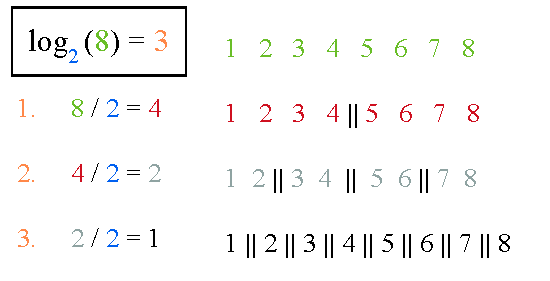
\includegraphics[width=.5\textwidth]{capitols/figures/log (4).pdf}
    \caption[Relació entre partir nombres i els logaritmes.]{Relació entre partir nombres i els logaritmes. Font: elaboració pròpia.}
    \label{fig:my_label}
\end{figure}
\vspace{-18pt}
Si el diccionari té $n$ pàgines i $n = 128$, seguint el procediment de l'exemple anterior, haurem de fer $\log_2{n} = \log_2{128} = 7$ passos per arribar a partir-lo en pàgines individuals.  Per això diem que la complexitat d'aquest algoritme és $O(\log_2{n})$.

Si representem aquesta complexitat en el gràfic 1.8, podem veure com quan la mida de l'entrada és més petita, el nombre d'operacions creix més ràpidament, però a mesura que les $n$ són més grans, cada vegada el nombre d'operacions creix més a poc a poc.
% ------------------------------gràfic complexitat log
\begin{figure}[H]
    \centering
\begin{tikzpicture}
\centering
\begin{axis}[xmin=0, xmax=100, ymin=0, ymax=40, axis lines = middle, 
x label style={at={(axis description cs:0.5,-0.1)},anchor=north},
y label style={at={(axis description cs:-0.1,.5)},rotate=90,anchor=south},
xlabel={$n$ mida de l'entrada},
ylabel={nombre d'operacions},
style={thick}, 
compat=1.18, width=.5\textwidth,
grid=both,
grid style={line width=.1pt, draw=gray!10},
major grid style={line width=.2pt,draw=gray!50},
    minor tick num=5
]
\addplot[color=vermellpral, domain=-2:100, samples=100]{log2(x)};
\legend{$O(\log_2{n})$}
\end{axis}
\end{tikzpicture}
    \caption[Complexitat logarítmica.]{Complexitat logarítmica. Font: elaboració pròpia.}
    \label{fig:my_label}
\end{figure}

Per tant, per a $n = 10$, farà $\log_2{n} = \lceil\log_2{10}\rceil = 4$ operacions i per a $n = 10^6$ farà $\log_2{n} = \lceil\log_2{10^6}\rceil = 20$ operacions.

\subsubsection*{Totes les complexitats}
Finalment, per comparar les diferents complexitats entre elles, podem fer un gràfic que les representi totes i una taula amb algunes dades per comparar-les. D'aquesta manera podem veure com la complexitat quadràtica té el cost més gran de les que hem explicat, i la complexitat logarítmica té menys cost excloent-hi la constant.

Els algoritmes de complexitat constant només es poden utilitzar per a problemes que no depenguin d'$n$, els quals són molt poc comuns i molt senzills, com per exemple operacions matemàtiques.

\begin{figure}[H]
    \centering
    \begin{tikzpicture}
    \begin{axis}[xmin=0, xmax=50, ymin=0, ymax=50, axis lines = middle,
    y label style={at={(axis description cs:-0.1,.5)},rotate=90,anchor=south},
    xlabel={$n$ mida de l'entrada},
    ylabel={nombre d'operacions},
    legend pos= outer north east,
    style={thick}, 
    compat=1.18, width=.65\textwidth, 
    grid=both,
grid style={line width=.1pt, draw=gray!10},
major grid style={line width=.2pt,draw=gray!50},
    minor tick num=5]
    \addplot[color=vermellpral, domain=0:200, samples=100]{1};
    \addplot[color=taronja, domain=-2:200, samples=200]{log2(x)};
    \addplot[color=verd, domain=0:200, samples=100]{x};
    \addplot[color=blau, domain=0:40, samples=200]{x^2};
\legend{$O(1)$,$O(log_{2}n)$, $O(n)$, $O(n^2)$}
    \end{axis}
    \end{tikzpicture}
    \caption[Gràfic amb totes les complexitats.]{Gràfic amb totes les complexitats. Font: elaboració pròpia.}
    \label{fig:my_label}
\end{figure}
\begin{figure}[H]
    \centering
    \begin{center}
    \renewcommand{\arraystretch}{1}
    \begin{tabular}{| l | * {5}{c|}}\hline
    \diagbox[width=.5\textwidth]{Complexitats}{$n$}
     & 10 & 1.000 & 10.000 & 50.000 & $10^{6}$ \\ 
     \hline
     \textit{$O(1)$} & 1 & 1 & 1 & 1 & 1 \\ 
     \hline
     \textit{$O(\log_2{n})$} & 4 & 10 & 14 & 16 & 20 \\
     \hline
     \textit{$O(n)$} & 10 & 1.000 & 10.000 & 50.000 & $10^{6}$ \\ 
    \hline
    \textit{$O(n^2)$} & 100 & $10^6$ & $10^8$ & $25 \cdot 10^8$ & $10^{12}$ \\ 
    \hline
    \end{tabular}
    \end{center}
    \caption[Taula amb exemples del nombre d'operacions per a cada  complexitat i mida d'entrada.]{Taula amb exemples del nombre d'operacions per a cada  complexitat i mida d'entrada. Font: elaboració pròpia.}
    \label{fig:my_label}
\end{figure}%

A més de les quatre complexitats elementals que hem explicat, n'hi ha més com la complexitat exponencial ($O(2^n)$) i la complexitat factorial ($O(n!)$) que tenen un cost molt superior a totes les altres. No les expliquem perquè no cal per als objectius d'aquest treball.


\section{Anàlisi d'algoritmes per a estructures de dades no lineals}
Les estructures de dades són diferents formes d'organitzar informació en un ordinador. En funció del programa que calgui implementar s'utilitzarà l'estructura de dades que sigui més convenient.

Depenent de l'estructura on guardem les dades per executar un algoritme, expressarem la complexitat amb diferents variables, ja que podem tenir diversos elements diferents com a entrada.

Les estructures de dades es classifiquen en dos tipus:
\begin{enumerate}
    \item Lineals. Per exemple: llistes, cues, piles i cues de prioritat.
    \item No lineals. Per exemple: grafs, arbres i taules hash.
\end{enumerate}

En aquest treball hem explicat tots els exemples utilitzant llistes, unes estructures lineals en què es poden guardar seqüències de nombres o paraules. Però hi ha altres algoritmes per a resoldre problemes més complexos en què és necessari utilitzar estructures no lineals. 

Per exemple, un problema molt important en la informàtica, és trobar el camí més curt entre dos punts. Guardar aquestes dades en una llista no és possible, per això hem d'utilitzar altres estructures de dades, en aquest cas un graf.

Un graf és un conjunt de vèrtex i arestes connectats entre elles. Els vèrtexs es representen amb cercles, i les arestes uneixen determinats vèrtexs. Es pot anar d'un vèrtex a un altre sempre que estiguin connectats per una aresta. El cost de passar per una aresta és 1 (excepte quan és un graf amb pesos a les arestes) i es pot anar en ambdues direccions si és un graf no dirigit com el de la figura 1.11, si no, s'anomena graf dirigit i les arestes es representen amb fletxes que indiquen el sentit.
\vspace{18pt}
\begin{figure}[H]
    \centering
    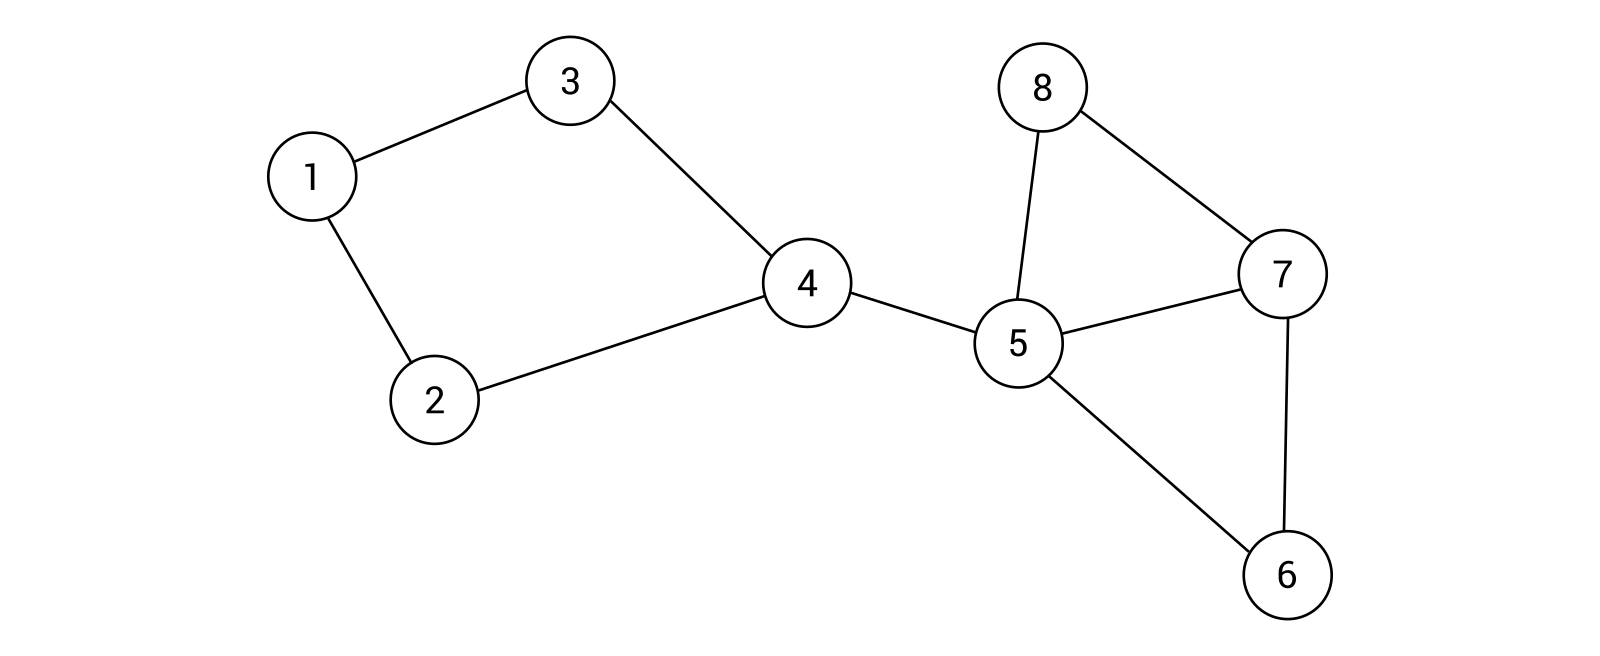
\includegraphics[width=.75\textwidth]{capitols/figures/7.png}
    \caption[Exemple de graf no dirigit i sense pesos a les arestes.]{Exemple de graf no dirigit i sense pesos a les arestes. Font: \\ https://www.oreilly.com/library/view/c-data-structures/9781788833738/0309b525-cfe4-429d-bdb9-53b25f94bbcd.xhtml.}
    \label{Figura}
\end{figure}

Per exemple, Google maps utilitza grafs per calcular el camí més curt entre dos llocs. Les interseccions són els vèrtexs i les carreteres les arestes. En aquest cas són grafs dirigits amb pesos a les arestes i calen algoritmes molt ràpids per recalcular el recorregut a l'instant.

També s'utilitzen grafs a les xarxes socials, els usuaris són vèrtex i els seguidors s'uneixen amb arestes, d'aquesta manera les xarxes socials poden suggerir nous seguidors.

No entrarem en detall, però problemes en què estructurem les dades en una estructura de dades no lineal, se segueixen analitzant en funció de la mida d'entrada, però la mida d'entrada no la podem definir com a $n$, ja que necessitem més variables.

En el cas dels grafs, analitzem la complexitat en funció de la quantitat nombre d'arestes ($A$) i vèrtexs ($V$) que hi ha. A diferència de les llistes, utilitzarem dues variables per definir la mida de l'entrada.

Hi ha molts algoritmes de grafs diferents per a resoldre problemes diferents, però hi ha dos algoritmes bàsics per a recórrer o travessar un graf sense pesos a les arestes, aquests són el breadth-first search o BFS (complexitat temporal d'$O(V + A)$) i depth-first search o DFS (complexitat temporal d'$O(V)$). I per grafs amb pesos l'algoritme bàsic és el Dijkstra (complexitat temporal d'$O((V + A)\log{V})$). Les implementacions d'aquests tres algoritmes les podeu trobar als annexos 6.2.

Aquests tres algoritmes són formes de recórrer el graf, és a dir, formes de visitar tots els vèrtexs de manera ordenada. Això és molt útil perquè variant una mica aquests algoritmes en funció del problema que es vulgui resoldre, es poden obtenir solucions a molts problemes diferents. Per això, tot i ser només formes d'iterar un graf, són algoritmes fonamentals per resoldre una gran varietat de problemes.

He fet una visualització de l'algoritme BFS implementat per a trobar el camí més curt entre dos punts en una matriu i el DFS implementat per indicar si hi ha un camí possible entre els dos punts de la matriu. Podeu trobar el programa en aquest enllaç: \url{https://github.com/JordinaGR/TDR-visualitzacio-BFS-DFS} o escanejant el codi de la figura 1.12.
\vspace{18pt}
\begin{figure}[H]
    \centering
    
\includegraphics[width=.15\textwidth]{capitols/figures/17.png}
    \caption[Programa de la visualització d'algoritmes de grafs.]{Programa de la visualització d'algoritmes de grafs. Font: elaboració pròpia.}
    \label{fig:my_label}
\end{figure}

He fet un vídeo que mostra el funcionament del programa, es pot trobar en el següent enllaç: \url{https://drive.google.com/file/d/1wqpY9PLo06W36MiOt74nirxrB-yl8TjB/view?usp=sharing} o escanejant el codi de la figura 1.13.
\begin{figure}[H]
    \centering
    
\includegraphics[width=.15\textwidth]{capitols/figures/16.png}
    \caption[Vídeo de la visualització d'algoritmes de grafs.]{Vídeo de la visualització d'algoritmes de grafs Font: elaboració pròpia.}
    \label{fig:my_label}
\end{figure}
